\chapter{Summary and Future Directions}
\label{ch7}


\section{Summary}

In this dissertation, we focus on the density estimation problem in an exponential family induced by a RKHS, $\calQ_{\ker}$. We proposed a new early stopping SM density estimator obtained via minimizing the (unpenalized) SM loss functional by the gradient descent algorithm and terminating early. We studied its statistical properties and compared it with the penalized SM density estimator in the literature and showed their similarities and differences. 

We also compared these two kinds of regularized SM density estimators with the penalized ML density estimator. Via numerical examples, we observed that the regularized SM density estimators are very sensitive to the presence of an isolated observation, especially when there is a small amount of regularization, but the penalized ML density estimator does \emph{not}. We attempted to explain why this happens. 

In order to understand this phenomenon, we extended the classic notion of the influence function to allow its input to be a function-valued statistical functional. Using this extended influence function, we studied the sensitivity of regularized SM and ML density estimators in both finite-dimensional and kernel exponential families. 

As we have mentioned at the end of the preceding chapter, we recommend to use the regularized SM density estimators, mainly due to its computational advantages. But when using them, one needs to make sure an appropriate amount of regularization has been imposed. 

% In this report, we have focused on the density estimation problem in $\calQ_{\ker}$ and the comparison of penalized ML, penalized SM, and early stopping SM density estimators. We also extend the notion of the influence function to study the sensitivity of these density estimators. We found that, even though regularized SM density estimators are easy to be computed, they are very sensitive to the presence of isolated observations, especially when the regularization is small. Penalized ML density estimator is hard to be computed but is less sensitive to the presence of isolated observations. 

\section{Future Directions}

Numerical examples shown in this dissertation are restricted to $d = 1$. We conjecture that regularized SM density estimators in higher dimensions ($d \ge 2$) are also very sensitive to the presence of an isolated observation when the regularization is small, and need numerical examples to confirm this. 

% Recently, the SM loss functional has been used in studying Gaussian graphical models \parencite{Forbes2015-pe}. We do not expect the sensitivity issue discussed in the preceding section occurs to these models, as the canonical statistics in these models are not local basis functions. However, it is interesting to go beyond the Gaussian graphical models and see whether the applications of the SM loss functional result in sensitivity issues in other types of graphical models. 

Several versions of generalized SM loss functionals have been proposed in the literature in recent years. \textcite{Parry2012-pa} proposed a version that does not only involve the first two derivatives of a log-density function but also the higher-order derivatives. \textcite{Yu2020-fb} proposed the following generalized H-divergence between $p_0$ and $q$ 
\begin{align}\label{eq-yu-hdiv}
	\int_{\calX} p_0 \parens{x} \norm[\big]{\nabla \log p_0 \parens{x} \odot \sqrt{h \parens{x}} - \nabla \log q \parens{x} \odot \sqrt{h \parens{x}} }_2^2 \diff x, 
\end{align}
where $\odot$ denotes element-wise multiplication of two vectors, $h: \calX \to [0, \infty)^d$, and the square root is taken element-wise. Under certain regularity conditions, one can apply integration by parts and obtain a loss functional from \eqref{eq-yu-hdiv} that depends on $q$ only. It is interesting to apply these generalized SM loss functionals to the density estimation problem in $\calQ_{\ker}$ and see whether the resulting density estimators are sensitive to the presence of an isolated observation. We conjecture, with an appropriate choice of $h$ in \eqref{eq-yu-hdiv}, the resulting density estimators may \emph{not} be very sensitive to isolated observations. 

%As we have discussed in Chapter \ref{ch1}, there has been an increasing interest in log-concave density estimation recently. The dominant approach is to minimize the NLL loss functional over the class of log-concave density functions over $\Real^d$, resulting in the ML log-concave density estimator. This approach leads to a non-differentiable objective function to optimize and involves approximations of the normalizing constant and its sub-gradient, which is computationally challenging. In addition, as is shown in Figure \ref{fig-logconcave-mle}, the ML log-concave density estimates contain ridges, and are only supported over the convex hull of data with all boundary points being the discontinuous points of the density estimate, which are undesirable qualitative features and may cause series issues in statistical applications. 
%
%Since the SM loss functional does not involve the normalizing constant and involves the first two partial derivatives of the log-density function, it is interesting to estimate a log-concave density function by minimizing the SM loss functional and compare the resulting SM log-concave density estimator with the ML log-concave density estimator. We conjecture the issues with the ML log-concave density estimator described above can be solved by using the SM loss functional. 
%
%\begin{figure}
%	\centering
%	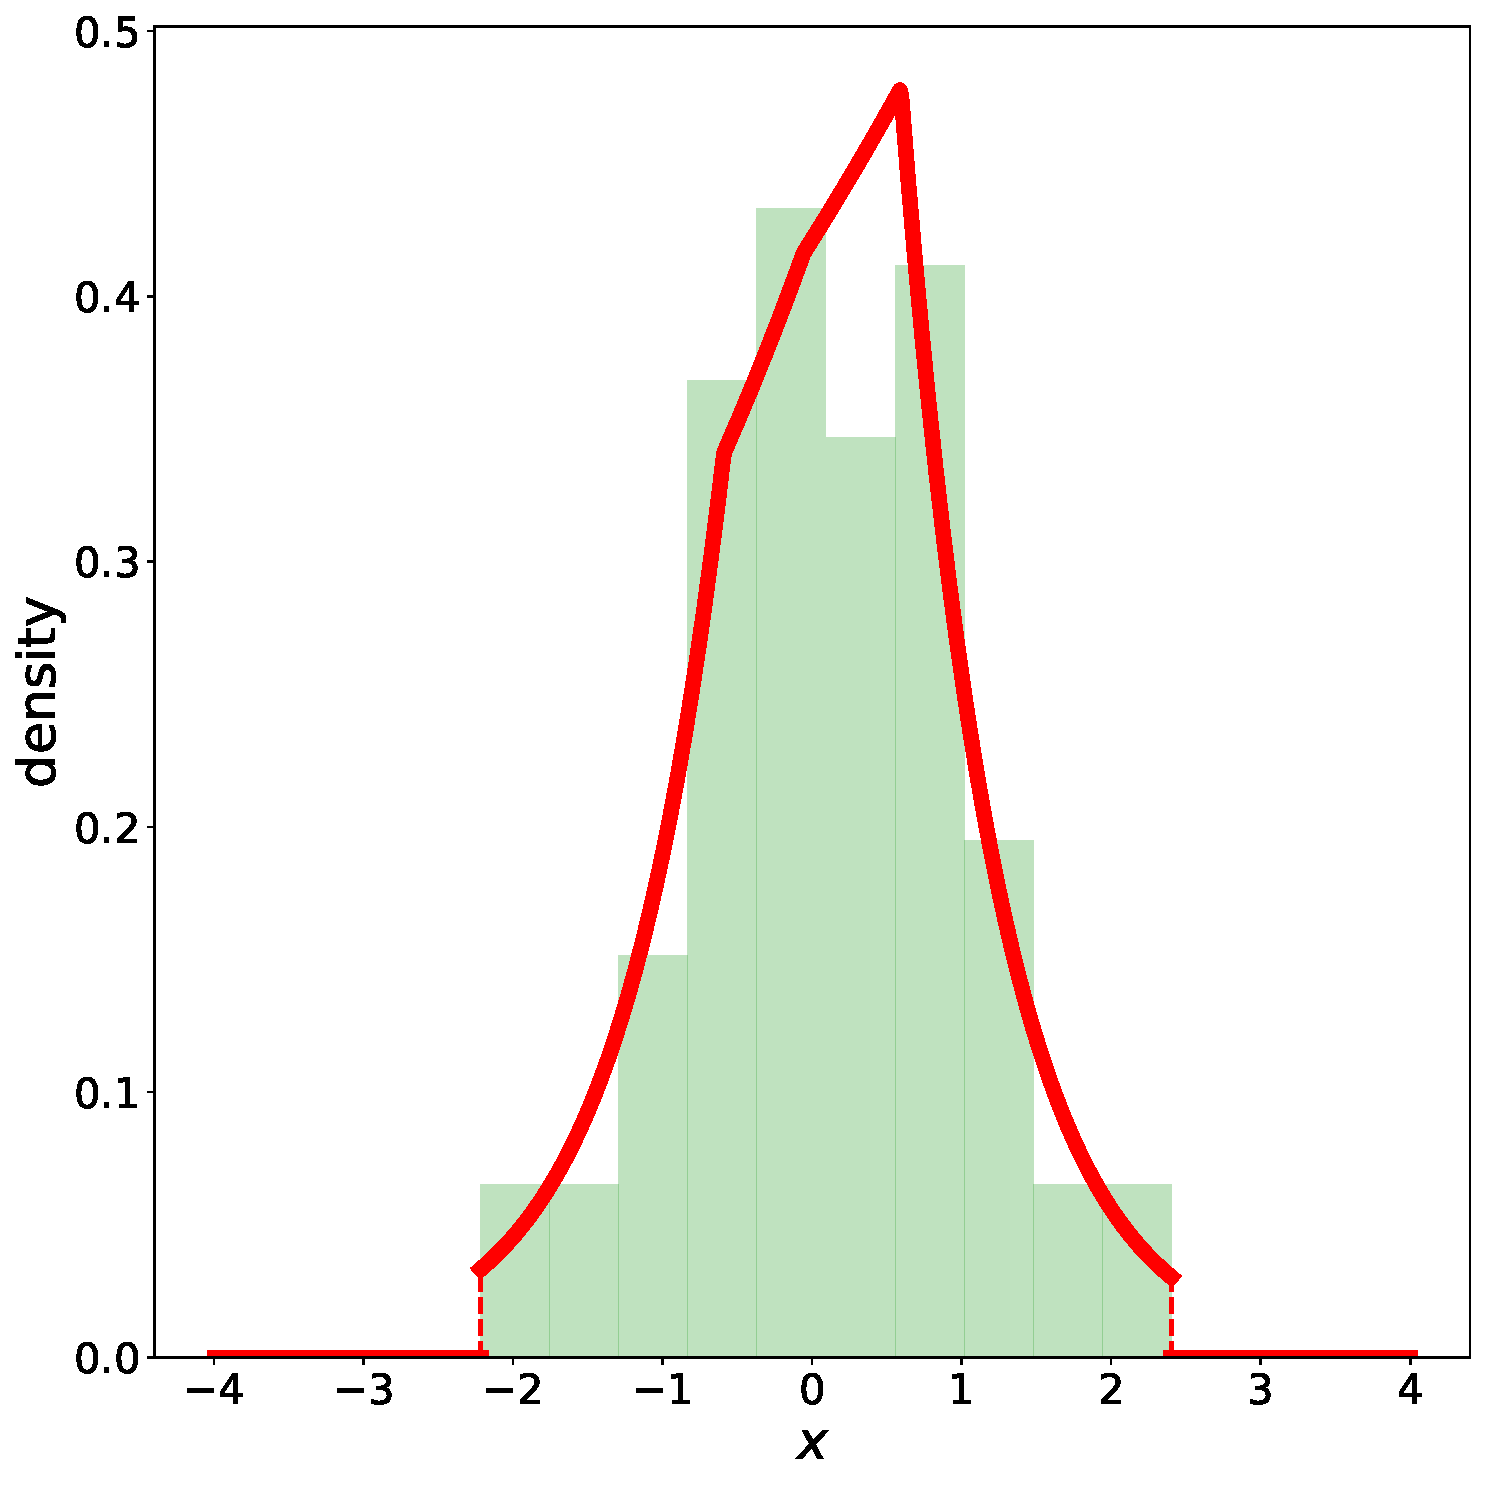
\includegraphics[width=0.6\textwidth]{../plots/log-concave-density-estimate-mle.pdf}
%	\caption{ML log-concave density estimate with 100 random samples from the standard normal distribution, where the density estimate is computed using the \texttt{R} package \texttt{logcondens} \parencite{Dumbgen2010-so}. Histogram with the bin width chosen by the Freedman-Diaconis rule is shown in green.}
%	\label{fig-logconcave-mle}
%\end{figure}
